\begin{landscape}

\begin{figure}
\begin{center}
{\scriptsize
\begin{tabular}{c|cccccc}
& \textbf{Jacobi(1)}&\textbf{Jacobi(8)}&\textbf{Jacobi(12)}&\textbf{Jacobi(16)}&\textbf{Jacobi(24)}&\textbf{Jacobi(32)}\\
\hline
\parbox[t]{2mm}{\multirow{1}{*}{\rotatebox[origin=r]{90}{\textbf{
    Jacobi(32)\hspace*{1.08cm}
    Jacobi(24)\hspace*{1.08cm}
    Jacobi(16)\hspace*{1.08cm}
    Jacobi(12)\hspace*{1.08cm}
    Jacobi(8)\hspace*{1.2cm}
    Jacobi(1)\hspace*{.5cm}}}}
}
\\

&
 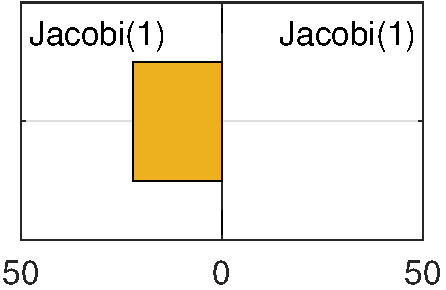
\includegraphics[width=.135\columnwidth]{plots/Jacobi(1)_vs_Jacobi(1).pdf}
&
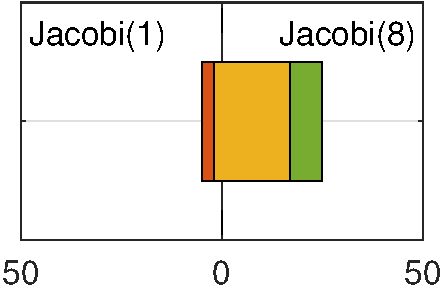
\includegraphics[width=.135\columnwidth]{plots/Jacobi(1)_vs_Jacobi(8).pdf}
&
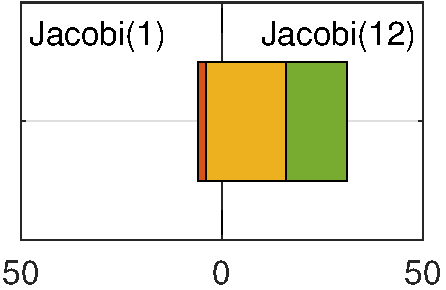
\includegraphics[width=.135\columnwidth]{plots/Jacobi(1)_vs_Jacobi(12).pdf}
&
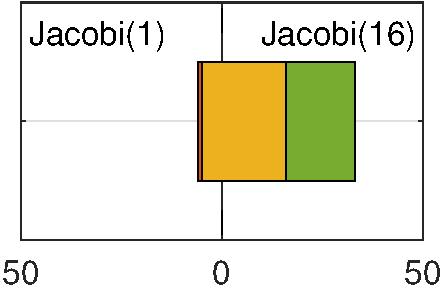
\includegraphics[width=.135\columnwidth]{plots/Jacobi(1)_vs_Jacobi(16).pdf}
&
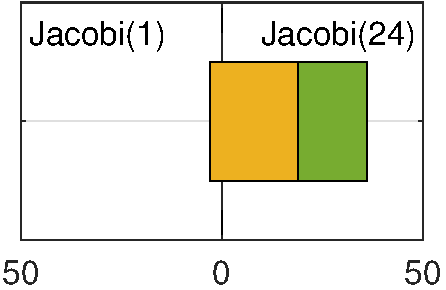
\includegraphics[width=.135\columnwidth]{plots/Jacobi(1)_vs_Jacobi(24).pdf}
&
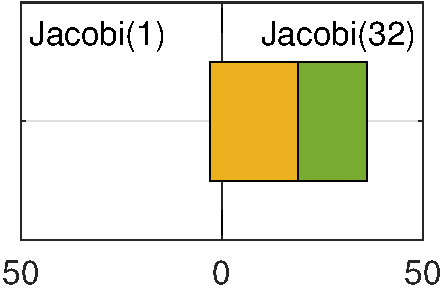
\includegraphics[width=.135\columnwidth]{plots/Jacobi(1)_vs_Jacobi(32).pdf}
\\
&
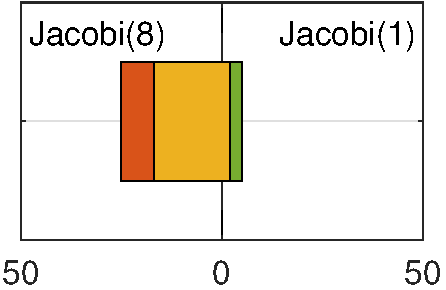
\includegraphics[width=.135\columnwidth]{plots/Jacobi(8)_vs_Jacobi(1).pdf}
&
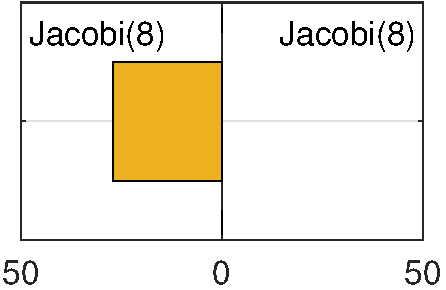
\includegraphics[width=.135\columnwidth]{plots/Jacobi(8)_vs_Jacobi(8).pdf}
&
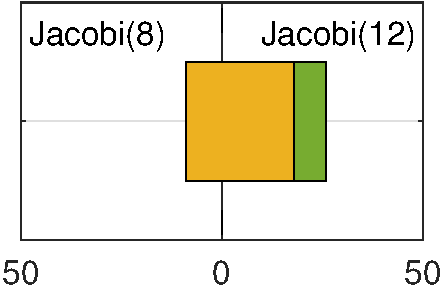
\includegraphics[width=.135\columnwidth]{plots/Jacobi(8)_vs_Jacobi(12).pdf}
&
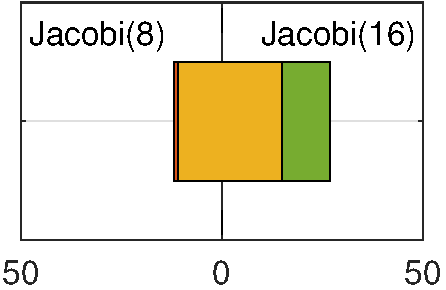
\includegraphics[width=.135\columnwidth]{plots/Jacobi(8)_vs_Jacobi(16).pdf}
&
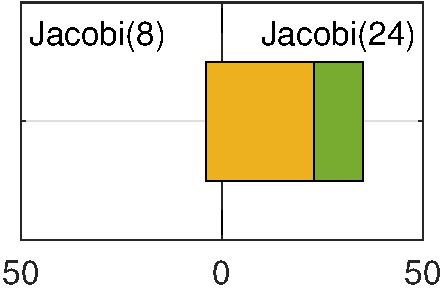
\includegraphics[width=.135\columnwidth]{plots/Jacobi(8)_vs_Jacobi(24).pdf}
&
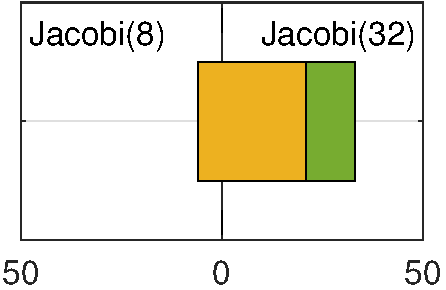
\includegraphics[width=.135\columnwidth]{plots/Jacobi(8)_vs_Jacobi(32).pdf}
\\
&
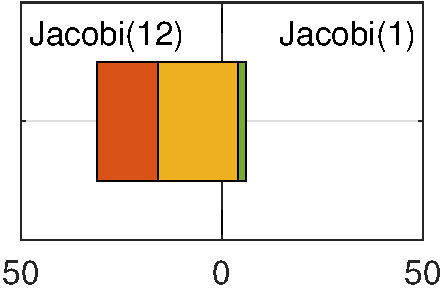
\includegraphics[width=.135\columnwidth]{plots/Jacobi(12)_vs_Jacobi(1).pdf}
&
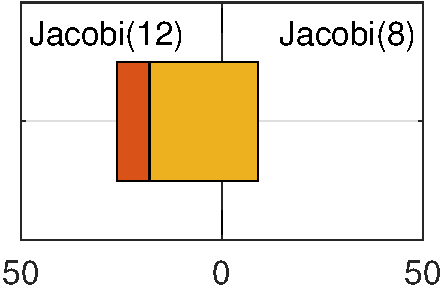
\includegraphics[width=.135\columnwidth]{plots/Jacobi(12)_vs_Jacobi(8).pdf}
&
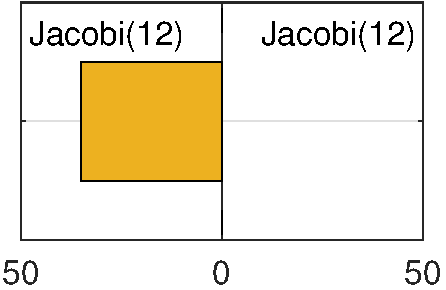
\includegraphics[width=.135\columnwidth]{plots/Jacobi(12)_vs_Jacobi(12).pdf}
&
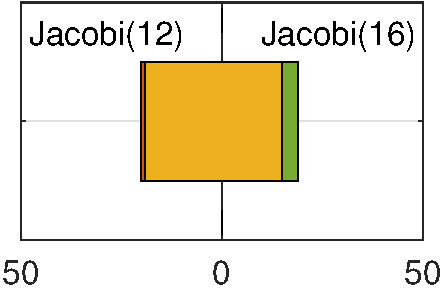
\includegraphics[width=.135\columnwidth]{plots/Jacobi(12)_vs_Jacobi(16).pdf}
&
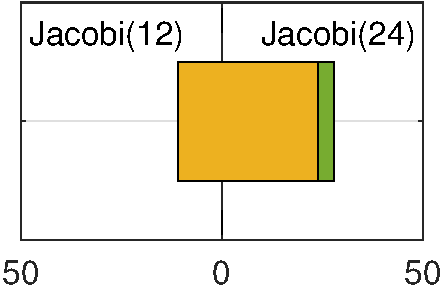
\includegraphics[width=.135\columnwidth]{plots/Jacobi(12)_vs_Jacobi(24).pdf}
&
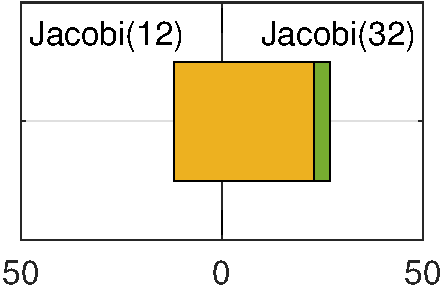
\includegraphics[width=.135\columnwidth]{plots/Jacobi(12)_vs_Jacobi(32).pdf}
\\
&
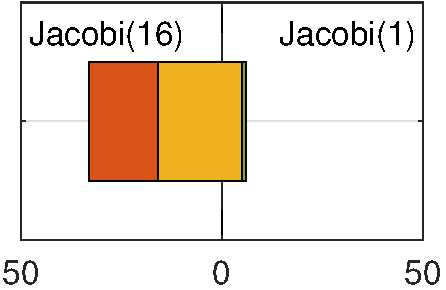
\includegraphics[width=.135\columnwidth]{plots/Jacobi(16)_vs_Jacobi(1).pdf}
&
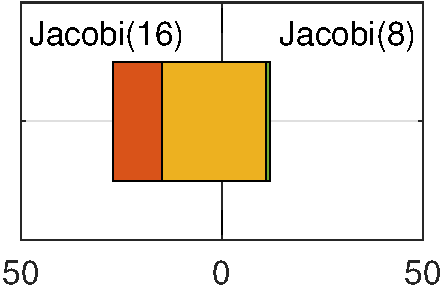
\includegraphics[width=.135\columnwidth]{plots/Jacobi(16)_vs_Jacobi(8).pdf}
&
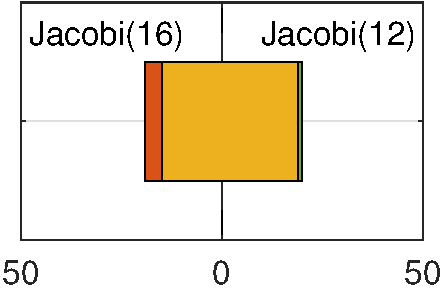
\includegraphics[width=.135\columnwidth]{plots/Jacobi(16)_vs_Jacobi(12).pdf}
&
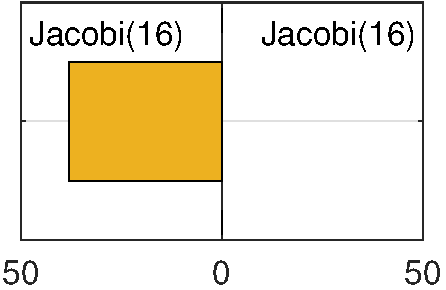
\includegraphics[width=.135\columnwidth]{plots/Jacobi(16)_vs_Jacobi(16).pdf}
&
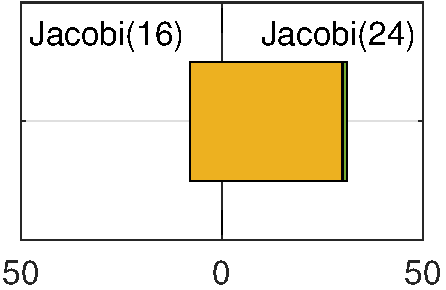
\includegraphics[width=.135\columnwidth]{plots/Jacobi(16)_vs_Jacobi(24).pdf}
&
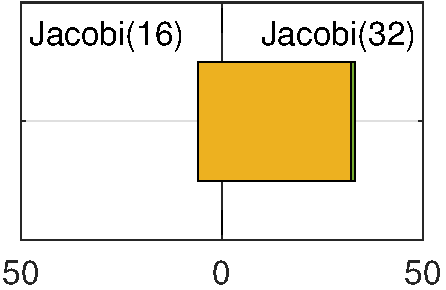
\includegraphics[width=.135\columnwidth]{plots/Jacobi(16)_vs_Jacobi(32).pdf}
\\
&
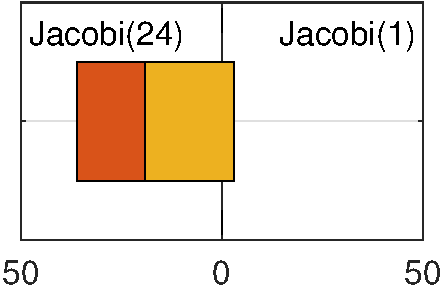
\includegraphics[width=.135\columnwidth]{plots/Jacobi(24)_vs_Jacobi(1).pdf}
&
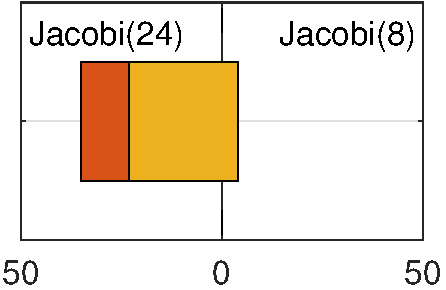
\includegraphics[width=.135\columnwidth]{plots/Jacobi(24)_vs_Jacobi(8).pdf}
&
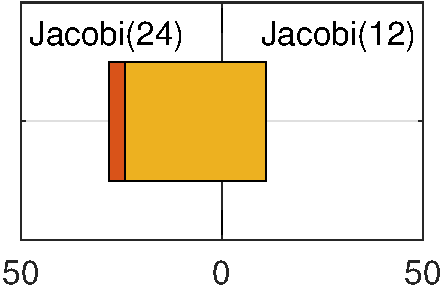
\includegraphics[width=.135\columnwidth]{plots/Jacobi(24)_vs_Jacobi(12).pdf}
&
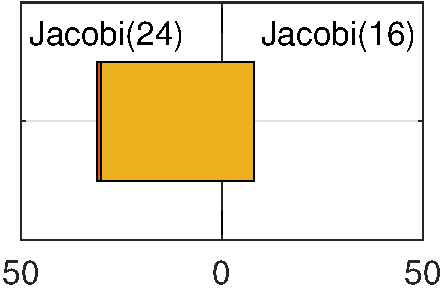
\includegraphics[width=.135\columnwidth]{plots/Jacobi(24)_vs_Jacobi(16).pdf}
&
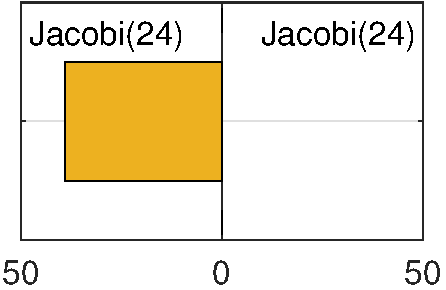
\includegraphics[width=.135\columnwidth]{plots/Jacobi(24)_vs_Jacobi(24).pdf}
&
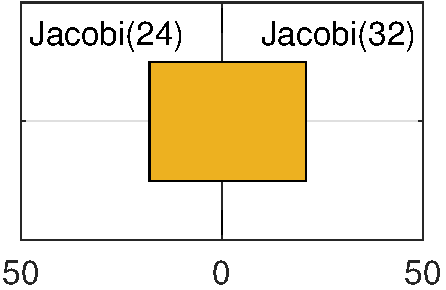
\includegraphics[width=.135\columnwidth]{plots/Jacobi(24)_vs_Jacobi(32).pdf}
\\
&
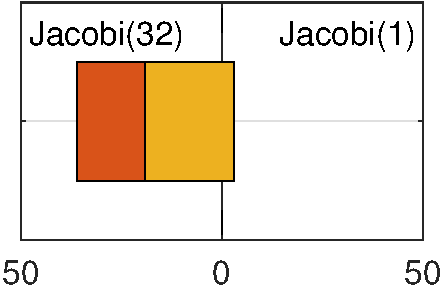
\includegraphics[width=.135\columnwidth]{plots/Jacobi(32)_vs_Jacobi(1).pdf}
&
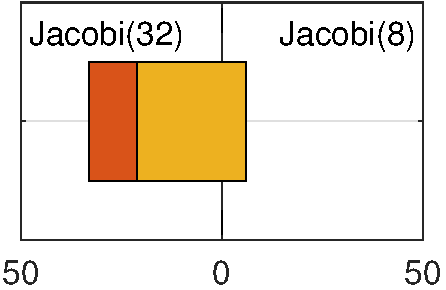
\includegraphics[width=.135\columnwidth]{plots/Jacobi(32)_vs_Jacobi(8).pdf}
&
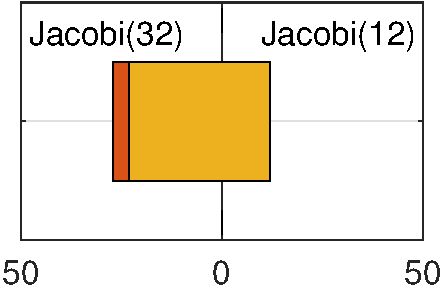
\includegraphics[width=.135\columnwidth]{plots/Jacobi(32)_vs_Jacobi(12).pdf}
&
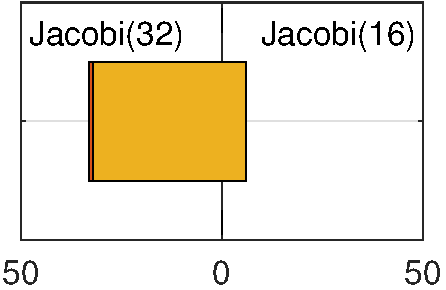
\includegraphics[width=.135\columnwidth]{plots/Jacobi(32)_vs_Jacobi(16).pdf}
&
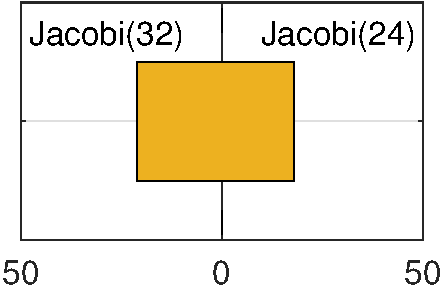
\includegraphics[width=.135\columnwidth]{plots/Jacobi(32)_vs_Jacobi(24).pdf}
&
 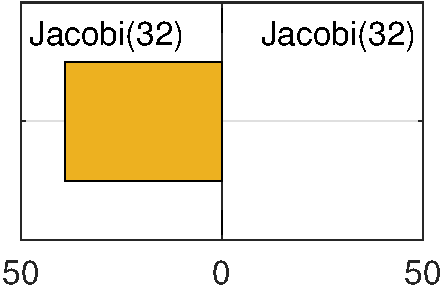
\includegraphics[width=.135\columnwidth]{plots/Jacobi(32)_vs_Jacobi(32).pdf}
\\
\end{tabular}
}
\end{center}
\caption
[Detailed comparison of IDR(4) enhanced with block-Jacobi
using different block sizes]
{
Detailed comparison of IDR(4) enhanced with block Jacobi
using different block sizes.
}
\label{2017-gje-block-jacobi:fig:solverperformance-detailed}
\end{figure}

\end{landscape}
\begin{landscape}
\begin{table}[p]
\scriptsize
\centering
\begin{tabular}{lrrr||rr|rr|rr|rr|rr|rr}
\hline
\hline
& & & & \multicolumn{2}{c|}{Jacobi} & \multicolumn{2}{c|}{Block-Jacobi (8)} &  \multicolumn{2}{c|}{Block-Jacobi (12)}
 & \multicolumn{2}{c|}{Block-Jacobi (16)}  & \multicolumn{2}{c|}{Block-Jacobi (24)} & \multicolumn{2}{c}{Block-Jacobi (32)}\\
 Matrix & size & \#nnz & ID & \#iters & time [s] & \#iters & time [s] & \#iters & time [s] & \#iters & time [s] & \#iters & time [s]  & \#iters & time [s]  \\
\hline
       ABACUS\_shell\_ud  &  23,412  &  218,484  &  26  &     3703 &     5.09  
       & \textbf{    2305} & \textbf{    3.32}  &     2829 &     4.09  &     
       3028 &     4.43  &     2858 &     4.27  &     2418 &     3.70\\
              bcsstk17  &  10,974  &  428,650  &  6  &     1967 &     2.87  
              &     1174 &     1.78  &      901 &     1.38  &      792 &     
              1.23  & \textbf{     735} & \textbf{    1.20}  &      879 &     
              1.40\\
              bcsstk18  &  11,948  &  149,090  &  39  &     1491 &     1.90  
              &      933 &     1.37  &      653 &     0.98  &      591 &     
              0.92  & \textbf{     440} & \textbf{    0.65}  &      532 &     
              0.85\\
              bcsstk38  &  8,032  &  355,460  &  10  &       --  &       --   
              &       --  &       --   &     2459 &     4.21  &     4290 &     
              7.33  & \textbf{    1878} & \textbf{    3.26}  &     2050 &     
              3.62\\
               cbuckle  &  13,681  &  676,515  &  9  &      434 &     0.81  
               &      118 &     0.22  & \textbf{      48} & \textbf{    0.11}  
               &      102 &     0.23  &       49 &     0.12  &       75 &     
               0.15\\
            Chebyshev2  &  2,053  &  18,447  &  5  &       --  &       --   
            &      197 &     0.53  &       62 &     0.18  &       53 &     
            0.15  &       38 &     0.11  & \textbf{      35} & \textbf{    
            0.10}\\
            Chebyshev3  &  4,101  &  36,879  &  17  &       --  &       --   
            &       --  &       --   &      194 &     0.67  &      177 &     
            0.66  &      113 &     0.40  & \textbf{      77} & \textbf{    
            0.31}\\
                   dc3  &  116,835  &  766,396  &  28  & \textbf{     168} & 
                   \textbf{   17.29}  &      169 &    17.36  &      203 &    
                   20.93  &      203 &    20.92  &      320 &    33.00  &      
                   183 &    18.87\\
                dw1024  &  2,048  &  10,114  &  30  &       --  &       --   
                &      169 &     0.23  &      148 &     0.27  &      163 &     
                0.30  &       92 &     0.18  & \textbf{      65} & \textbf{    
                0.13}\\
                dw2048  &  2,048  &  10,114  &  7  &       --  &       --   
                &      169 &     0.23  &      148 &     0.27  &      163 &     
                0.30  &       92 &     0.17  & \textbf{      65} & \textbf{    
                0.12}\\
                dw4096  &  8,192  &  41,746  &  18  &       --  &       --   
                &       --  &       --   &       --  &       --   &     6949 
                &     8.96  &     1732 &     2.33  & \textbf{    1012} & 
                \textbf{    1.46}\\
                dw8192  &  8,192  &  41,746  &  36  &       --  &       --   
                &       --  &       --   &       --  &       --   &     6949 
                &     8.94  &     1732 &     2.35  & \textbf{    1012} & 
                \textbf{    1.41}\\
                    F1  &  343,791  &  26,837,113  &  27  &     3832 &    
                    23.93  &       --  &       --   &     2460 &    16.34  
                    &     2511 &    17.00  & \textbf{    1895} & \textbf{   
                    13.23}  &     2062 &    14.78\\
            G3\_circuit  &  1,585,478  &  7,660,826  &  31  &     2346 &    
            19.94  & \textbf{    2069} & \textbf{   19.52}  &     2220 &    
            22.14  &     1935 &    20.09  &     2085 &    24.10  &     2198 
            &    26.83\\
              gridgena  &  48,962  &  512,084  &  32  &     2265 &     3.51  
              &     1306 &     2.08  &     1766 &     2.84  &     1431 &     
              2.33  & \textbf{    1028} & \textbf{    1.70}  &     1311 &     
              2.26\\
          ibm\_matrix\_2  &  51,448  &  537,038  &  21  &       --  &       
          --   &       --  &       --   & \textbf{     227} & \textbf{    
          0.46}  &     8992 &    17.45  &      254 &     0.55  &     2965 &     
          6.04\\
                   Kuu  &  7,102  &  340,200  &  3  &      162 &     0.29  
                   &      103 &     0.19  &       95 &     0.18  & 
                   \textbf{      84} & \textbf{    0.16}  &       94 &     
                   0.18  &       84 &     0.17\\
        LeGresley\_2508  &  2,508  &  16,727  &  20  &      237 &     0.40  
        &      247 &     0.36  &      203 &     0.35  &       --  &       --   
        &      185 &     0.33  & \textbf{     166} & \textbf{    0.31}\\
              linverse  &  11,999  &  95,977  &  35  &     6185 &     7.80  
              &       --  &       --   &       --  &       --   &     6685 
              &     9.51  &     2175 &     3.07  & \textbf{     933} & 
              \textbf{    1.44}\\
              matrix\_9  &  103,430  &  1,205,518  &  2  &     1512 &     2.72  
              &      727 &     1.37  &       95 &     0.21  &      598 &     
              1.18  & \textbf{      87} & \textbf{    0.20}  &      558 &     
              1.16\\
              nasa2910  &  2,910  &  174,296  &  12  &      738 &     1.03  
              &      529 &     0.73  &      509 &     0.74  &      648 &     
              0.94  &      435 &     0.67  & \textbf{     392} & \textbf{    
              0.64}\\
                 nd12k  &  36,000  &  14,220,946  &  19  &       --  &       
                 --   &     6869 &    20.67  &     3183 &     9.67  &     2764 
                 &     8.45  & \textbf{    1543} & \textbf{    4.81}  &     
                 1693 &     5.35\\
                 nd24k  &  72,000  &  28,715,634  &  11  &       --  &       
                 --   &     4918 &    23.29  &     2906 &    13.85  &     2858 
                 &    13.69  &     1916 &     9.35  & \textbf{    1457} & 
                 \textbf{    7.16}\\
                  nd3k  &  9,000  &  3,279,690  &  33  &       --  &       --   
                  &       --  &       --   &     4551 &     8.05  &     8270 
                  &    14.55  & \textbf{    2640} & \textbf{    4.78}  &     
                  3196 &     5.87\\
                  nd6k  &  18,000  &  6,897,316  &  29  &       --  &       
                  --   &       --  &       --   &     5142 &    11.14  &     
                  9178 &    19.94  & \textbf{    2589} & \textbf{    5.76}  
                  &     2573 &     5.81\\
              nemeth15  &  9,506  &  539,802  &  34  &       94 &     0.17  
              &       --  &       --   &       --  &       --   &      144 
              &     0.27  &       50 &     0.10  & \textbf{      49} & 
              \textbf{    0.10}\\
               olm5000  &  5,000  &  19,996  &  15  &       --  &       --   
               &     1164 &     1.58  &     1049 &     1.44  &      256 &     
               0.41  &      545 &     0.80  & \textbf{     178} & \textbf{    
               0.33}\\
          Pres\_Poisson  &  14,822  &  715,804  &  4  &      199 &     0.38  
          &      130 &     0.24  &      129 &     0.26  &      113 &     0.23  
          &       93 &     0.19  & \textbf{      82} & \textbf{    0.17}\\
            rail\_79841  &  79,841  &  553,921  &  1  &      995 &     1.62  
            &      909 &     1.56  &     1013 &     1.78  & \textbf{     880} & 
            \textbf{    1.52}  &      862 &     1.58  &      810 &     1.52\\
              s1rmt3m1  &  5,489  &  217,651  &  22  &      296 &     0.43  
              &      191 &     0.32  & \textbf{     171} & \textbf{    0.24}  
              &      159 &     0.28  &      148 &     0.28  &      148 &     
              0.27\\
              s2rmq4m1  &  5,489  &  263,351  &  37  &      708 &     0.97  
              &      231 &     0.39  & \textbf{     223} & \textbf{    0.36}  
              &      262 &     0.43  &      214 &     0.36  &      198 &     
              0.36\\
              s2rmt3m1  &  5,489  &  217,681  &  25  &     1016 &     1.35  
              &      327 &     0.50  &      209 &     0.35  &      218 &     
              0.36  & \textbf{     178} & \textbf{    0.32}  &      220 &     
              0.40\\
              s3rmq4m1  &  5,489  &  262,943  &  24  &       --  &       --   
              &     1387 &     1.95  &      599 &     0.89  &     1969 &     
              2.83  & \textbf{     515} & \textbf{    0.80}  &      972 &     
              1.47\\
              s3rmt3m1  &  5,489  &  217,669  &  16  &       --  &       --   
              &       --  &       --   &      693 &     0.99  &     2637 &     
              3.62  & \textbf{     529} & \textbf{    0.75}  &     1142 &     
              1.71\\
              s3rmt3m3  &  5,357  &  207,123  &  23  &       --  &       --   
              &       --  &       --   &     1995 &     2.74  &     2087 &     
              2.86  &     2229 &     3.14  & \textbf{     784} & \textbf{    
              1.18}\\
                saylr4  &  3,564  &  22,316  &  38  &     1907 &     2.46  
                &      387 &     0.59  &      246 &     0.40  &      281 &     
                0.38  & \textbf{     163} & \textbf{    0.30}  &      170 &     
                0.32\\
              ship\_003  &  121,728  &  3,777,036  &  13  &       --  &       
              --   &     2058 &     4.89  &     1927 &     4.62  &     2849 
              &     6.97  & \textbf{    1683} & \textbf{    4.26}  &     2160 
              &     5.75\\
                sme3Dc  &  42,930  &  3,148,656  &  8  & \textbf{    2680} & 
                \textbf{    5.66}  &     4953 &    10.59  &     3101 &     
                6.74  &     3014 &     6.53  &     3566 &     7.92  &     4990 
                &    11.19\\
               sts4098  &  4,098  &  72,356  &  14  &      135 &     0.26  
               &      113 &     0.23  &       78 &     0.12  &       94 &     
               0.19  &       76 &     0.16  & \textbf{      64} & \textbf{    
               0.11}\\
\hline
\hline
\end{tabular}

\captionsetup{width=\textwidth}
\caption
[Iterations and execution time of IDR(4) enhanced with GJE-based block-Jacobi]
{Iterations and execution time of IDR(4) enhanced with scalar Jacobi
preconditioning or block-Jacobi preconditioning.
The runtime combines the preconditioner setup time and the iterative solver execution time.
}
\label{2017-gje-block-jacobi:tab:idr4comparison}
\end{table}

\end{landscape}
